\documentclass[pra,12pt]{revtex4}
\usepackage{amsmath}
\usepackage{amssymb}
\usepackage{graphicx}
\usepackage{color}
\usepackage[pdfborder={0 0 0},colorlinks=true,linkcolor=blue,urlcolor=blue]{hyperref}

\def\ket#1{\left|#1\right\rangle}
\def\bra#1{\left\langle#1\right|}
\def\braket#1{\left\langle#1\right\rangle}

\usepackage{fancyhdr}
\fancyhf{}
\lhead{\tiny Y.~D.~Chong}
\rhead{\scriptsize PH4401: Quantum Mechanics III}
\lfoot{}
\rfoot{\thepage}
\pagestyle{fancy}

\setlength{\parindent}{14pt}
\renewcommand{\theequation}{A.\arabic{equation}}
\renewcommand{\thesection}{A\arabic{section}}

\renewcommand{\baselinestretch}{1.0}
\setlength{\parskip}{0.04in}

\begin{document}

\begin{center}
{\large \textbf{Appendix A: Circular and Spherical Waves}}
\end{center}

This Appendix describes the mathematics of circular waves and
spherical waves, and their use in 2D and 3D scattering problems.

\section{The Helmholtz equation}

Consider a non-relativistic particle moving in $d$-dimensional space
in the absence of a potential ($V = 0$), as in the exterior region of
a scattering problem (Chapter 1).  The time-independent Schr\"odinger
equation is
\begin{equation}
  -\frac{\hbar^2}{2m}\nabla^2 \psi(\mathbf{r}) = E \psi(\mathbf{r}),
  \label{tise}
\end{equation}
where $\nabla^2$ denotes the $d$-dimensional Laplacian.  We assume $E
> 0$, and focus on the $d = 2$ and $d = 3$ cases.

It is convenient to rewrite Eq.~\eqref{tise} as
\begin{equation}
  \Big(\nabla^2 + k^2\Big) \psi(\mathbf{r}) = 0,
  \label{helmholtz}
\end{equation}
where
\begin{equation}
  k = \sqrt{\frac{2mE}{\hbar^2}} \;\in\; \mathbb{R}^+.
  \label{kparm}
\end{equation}
The partial differential equation \eqref{helmholtz} is called the
\textbf{Helmholtz equation}.  We are interested in its solutions for
various choices of boundary conditions, in both 2D and 3D space.

One class of elementary solutions is, of course, the plane waves
\begin{equation}
  \psi(\mathbf{r}) = \psi_0 \, \exp\left(i\mathbf{k}\cdot\mathbf{r}\right),
  \label{planewaves}
\end{equation}
where $\psi_0 \in \mathbb{C}$ and $\mathbf{k}$ is a $d$-component
vector satisfying $|\mathbf{k}| = k$.  The direction of $\mathbf{k}$
specifies the propagation direction.

In scattering problems, it is useful to consider other solutions that
correspond to waves propagating outward (or inward) from a point,
unlike a plane wave.  Such solutions can be constructed using polar
coordinates $(r, \phi)$ in 2D, and spherical coordinates
$(r,\theta,\phi)$ in 3D.

\section{Circular Waves in 2D}
\label{circular_waves}

In 2D polar coordinates $(r, \phi)$, the wavefunction has the form
\begin{equation}
  \psi(\mathbf{r}) = \psi(r,\phi).
\end{equation}
Since $\phi$ is an angular variable---i.e., $\psi(r,\phi + 2\pi) =
\psi(r, \phi)$---we can simplify the $\phi$ dependence by focusing on
harmonic solutions
\begin{equation}
  \psi(r,\phi) = \Psi_m(r)\, e^{im\phi}, \;\;\;m \in\mathbb{Z}.
  \label{psi_circular}
\end{equation}
More general solutions can be constructed from these, using
superpositions of different $m$.

By plugging Eq.~\eqref{psi_circular} into the Helmholtz equation
\eqref{helmholtz}, and expressing the 2D Laplacian in polar
coordinates, we arrive at the following ordinary differential equation
for $\Psi_m(r)$:
\begin{equation}
  r \frac{d}{dr}\!\left(r \frac{d\Psi_m}{dr} \right)
  + \Big(k^2 r^2 - m^2 \Big)\, \Psi_m(r) = 0.
  \label{besseleq}
\end{equation}
This is the \textbf{Bessel equation}, which supports the following
solutions:
\begin{equation}
  \Psi_m(r) \propto \begin{cases}
    J_m(kr) &\text{\small(\href{https://docs.scipy.org/doc/scipy/reference/generated/scipy.special.jv.html}{Bessel function of the 1st kind})} \\
    Y_m(kr) &\text{\small(\href{https://docs.scipy.org/doc/scipy/reference/generated/scipy.special.yv.html}{Bessel function of the 2nd kind})} \\
    H_m^+(kr) \equiv J_m(kr) + i Y_m(kr) &\text{\small(\href{https://docs.scipy.org/doc/scipy/reference/generated/scipy.special.hankel1.html}{Hankel function of the 1st kind})} \\
    H_m^-(kr) \equiv J_m(kr) - i Y_m(kr) &\text{\small(\href{https://docs.scipy.org/doc/scipy/reference/generated/scipy.special.hankel2.html}{Hankel function of the 2nd kind})}.
  \end{cases}
\end{equation}
(Click on the links to refer to the implementations of these functions
in \href{https://scipy.org/}{Scientific Python}.)  The $J_m$ and $Y_m$
functions are real, while the $H_m^\pm$ functions are complex.
Notably, these four functions satisfy different boundary conditions:

\begin{itemize}
\item For $kr \rightarrow 0$, $J_m(kr)$ is finite, while the others ($Y_m$ and
$H_m^\pm$) are divergent.

\item For $kr \rightarrow \infty$, they have the following asymptotic forms:
\end{itemize}
\vskip -0.26in
\begin{align}
  \left.
  \begin{aligned}
    J_m(kr) &\rightarrow
    \sqrt{\frac{2}{\pi kr}} \cos\!\left(kr - \frac{m\pi}{2} - \frac{\pi}{4}\right) \\
    Y_m(kr) &\rightarrow
    \sqrt{\frac{2}{\pi kr}} \sin\!\left(kr - \frac{m\pi}{2} - \frac{\pi}{4}\right) \\
    H_m^\pm(kr) &\rightarrow
    \sqrt{\frac{2}{\pi kr}}
    \exp\left[\pm i\left(kr - \frac{m\pi}{2} - \frac{\pi}{4}\right)\right] \\
  \end{aligned}\;\;
  \right\}
  \; \text{for}\;\, -\pi < \mathrm{arg}[kr] < \pi.
  \label{Jasymptote}
\end{align}

By looking at the last line in Eq.~\eqref{Jasymptote} and drawing an
analogy to Eq.~\eqref{planewaves}, we see that the Hankel functions of
the first kind describe \textit{outgoing} waves (propagating away from
the origin), and the Hankel functions of the second kind describe
\textit{incoming} waves (propagating toward the origin).  The
prefactor of $1/\sqrt{r}$ is consistent with energy conservation: in
2D, the wavefront at radius $r$ has circumference $2\pi r$, so
$|\Psi_m(r)|^2 \cdot 2\pi r$ is a constant.

\begin{figure}[b]
  \centering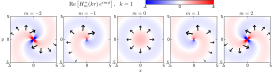
\includegraphics[width=0.99\textwidth]{bessels}
\end{figure}

The figure below plots the outgoing wavefunctions $H_m^+(kr) \,
\exp(im\phi)$ for different $m$.  Since the wavefunction is complex,
we plot just its real part, using red and blue to represent positive
and negative values.  The radial factor $H_m^+(kr)$ produces an
overall outward motion, while the $\exp(im\phi)$ factor describes the
azimuthal motion.  The black arrows indicate the wave's direction of
propagation at different points, showing that it spirals clockwise
outward ($m < 0$), propagates istropically outward ($m \ne 0$), or
spirals counterclockwise outward ($m > 0$).  Note that the $m = 0$
plot has no apparent divergence at $r = 0$ because we are plotting the
real part of the wavefunction, and the divergence of $H_m^+$ is in its
imaginary part (i.e., from $Y_m$).

We can then interpret the Bessel functions of the first and second
kind as superpositions of $H_m^+$ and $H_m^-$, similar to how standing
waves are superpositions of counter-propagating plane waves.  The
$J_m$ functions consist of a superposition that is non-divergent at $r
= 0$, because the divergences of $H_m^+$ and $H_m^-$ cancel out.  The
$Y_m$ functions are formed by a superposition that is divergent at $r
= 0$.

Finally, it is important to bear in mind that plane waves and circular
waves are both equally valid classes of elementary solutions to the 2D
Helmholtz equation.  We can even express a plane wave as a
superposition of circular waves, or vice versa.  The following
identity is particularly helpful for translating between the two types
of waves:
\begin{equation}
  e^{ikr\cos\phi} = \sum_{m=-\infty}^\infty i^m e^{im\phi} \, J_m(kr).
  \label{eikrcosphi}
\end{equation}
Its usefulness will be demonstrated in Section~\ref{sec:scattering}.

\section{Spherical Waves in 3D}
\label{sec:spherical}

In 3D, we can adopt spherical coordinates $(r, \theta, \phi)$.  To
solve the 3D Helmholtz equation, we can simplify the dependence on
$\theta$ and $\phi$ by focusing on solutions of the form
\begin{equation}
  \psi(r,\theta,\phi) = \Psi_{\ell m}(r) \,Y_{\ell m}(\theta, \phi),
  \label{psi3d}
\end{equation}
where $Y_{\ell m}(\theta,\phi)$ is a
\href{https://docs.scipy.org/doc/scipy/reference/generated/scipy.special.sph_harm.html}{spherical
  harmonic}.  In the quantum context, Eq.~\eqref{psi3d} describes a
wavefunction with definite angular momentum, described by the quantum
numbers $\ell$ (for the total angular momentum) and $m$ (for the
$z$-component of the angular momentum), which are integers satisfying
\begin{equation}
  \ell \ge 0 \;\;\mathrm{and}\; -\ell\le m \le \ell.
\end{equation}
This ensures that $Y_{\ell m}(\theta,\phi)$ is periodic in $\phi$ and
regular at the coordinate poles.

Plugging Eq.~\eqref{psi3d} into the Helmholtz equation, and expressing
the 3D Laplacian in spherical coordinates, yields
\begin{equation}
  \frac{d}{dr}\left(r^2 \, \frac{d\Psi_{\ell m}}{dr}\right)
  + \Big[k^2r^2 - \ell(\ell+1)\Big] \Psi_{\ell m}(r) = 0.
  \label{sphbessel}
\end{equation}
Remarkably, the differential equation involves $\ell$ but \textit{not}
$m$.  The solution thus only depends on $\ell$, and we henceforth
write it as $\Psi_\ell(r)$.  Now, Eq.~\eqref{sphbessel} has the
following solutions:
\begin{equation}
  \Psi_\ell(r) \propto \begin{cases}
    j_\ell(kr) &\text{\small(\href{https://docs.scipy.org/doc/scipy/reference/generated/scipy.special.spherical_jn.html}{Spherical Bessel function of the 1st kind})} \\
    y_\ell(kr) &\text{\small(\href{https://docs.scipy.org/doc/scipy/reference/generated/scipy.special.spherical_yn.html}{Spherical Bessel function of the 2nd kind})} \\
    h_\ell^+(kr) \equiv j_\ell(kr) + i y_\ell(kr) &\text{\small(\href{}{Spherical Hankel function of the 1st kind})} \\
    h_\ell^-(kr) \equiv j_\ell(kr) - i y_\ell(kr) &\text{\small(\href{}{Spherical Hankel function of the 2nd kind})}.
  \end{cases}
\end{equation}
Their boundary behaviors are closely analogous to the 2D counterparts
from Section~\ref{circular_waves}:

\begin{itemize}
\item For $kr \rightarrow 0$, $j_\ell(kr)$ is finite, while the others
  ($y_\ell$ and $h_\ell^\pm$) are divergent.

\item For $kr \rightarrow \infty$, they have the following asymptotic forms:
\end{itemize}
\vskip -0.2in
\begin{align}
  \left.
  \begin{aligned}
    j_\ell(kr)\; &\rightarrow \; \frac{\sin(kr-\frac{\ell\pi}{2})}{kr} \\
    y_\ell(kr)\; &\rightarrow \; - \frac{\cos(kr-\frac{\ell\pi}{2})}{kr} \\
    h_\ell^\pm(kr)\; &\rightarrow \; \pm \frac{\exp\left[\pm i(kr-\frac{\ell\pi}{2})\right]}{ikr}
  \end{aligned}\;\;
  \right\}
  \; \text{for}\;\, -\pi < \mathrm{arg}[kr] < \pi.
  \label{sphJasymptote}
\end{align}
Hence, the spherical Hankel functions of the first and second kind
describe outgoing and incoming waves, respectively.  The $1/r$
prefactors are consistent with energy conservation: in 3D, spherical
wavefronts are spread over an area $4\pi r^2$, so $|\Psi_{\ell
  m}(r)|^2 \cdot 4\pi r^2$ is a constant.

Similar to the 2D case, we can express a plane wave as a superposition
of spherical waves.  This is accomplished via the identity
\begin{equation}
  e^{i\mathbf{k}_i \cdot \mathbf{r}}
  = \sum_{\ell=0}^\infty \sum_{m=-\ell}^\ell 4 \pi j_{\ell}(kr) e^{i\ell\pi/2} \,
  Y_{\ell m}^*(\hat{\mathbf{k}}_i) \, Y_{\ell m}(\hat{\mathbf{r}}),
  \label{plane_wave_decomp}
\end{equation}
where $\hat{\mathbf{k}}_i$ denotes the angular components (in
spherical coordinates) of the incident wave-vector $\mathbf{k}_i$, and
$\hat{\mathbf{r}}$ denotes the angular components of the position
vector $\mathbf{r}$.

\section{Propagators}
\label{sec:propagator}

As discussed in Section 1.7, a propagator is a Green's function for a
free particle, meaning that it is a solution to
\begin{equation}
  \Big(\nabla^2 + k^2\Big) \langle\mathbf{r} |\hat{G}_0 |\mathbf{r}'\rangle
  = \frac{2m}{\hbar^2} \; \delta^d(\mathbf{r}-\mathbf{r}').
  \label{greendelta}
\end{equation}
The left side of this equation is the same as the $d$-dimensional
Helmholtz equation \eqref{helmholtz}, with $\nabla^2$ acting on
$\mathbf{r}$ (not $\mathbf{r}'$), and $k$ given by Eq.~\eqref{kparm}.
On the right side, $\delta^d(\cdots)$ denotes a $d$-dimensional delta
function, and the prefactor of $2m/\hbar^2$ comes from our definition
of the Green's function in terms of inverting the Hamiltonian (Section
1.6).

We can solve Eq.~\eqref{greendelta} with the help of the momentum
eigenbasis:
\begin{align}
  \langle\mathbf{r}|\hat{G}_0|\mathbf{r}'\rangle
  &= \langle\mathbf{r}|\hat{G}_0 \Big(\int d^dk' |\mathbf{k}'\rangle\langle\mathbf{k}'| \Big) |\mathbf{r}'\rangle \nonumber \\
  &= \int d^dk' \; \langle\mathbf{r}|\mathbf{k}'\rangle \;
  \frac{1}{E-\frac{\hbar^2|\mathbf{k}'|^2}{2m}} \;
  \langle\mathbf{k}'|\mathbf{r}'\rangle \nonumber \\
  &= \frac{2m}{\hbar^2} \frac{1}{(2\pi)^d} \int d^dk' \;
  \frac{\exp\left[i\mathbf{k}' \cdot
      (\mathbf{r}-\mathbf{r}')\right]}{k^2-|\mathbf{k}'|^2}.
  \label{rGr}
\end{align}
To calculate the $d$-dimensional integral, we must introduce explicit
coordinates.  In the following, we will show the calculation for 3D.
The 2D case is left as an \hyperref[ex:2dpropagator]{exercise}.

\clearpage

In 3D, let us express $\mathbf{k}'$ using spherical coordinates
$(k',\theta,\phi)$.  We are free to choose the $\theta=0$ axis so that
it points in the direction of $\mathbf{r}-\mathbf{r}'$, as illustrated
below:

\begin{figure}[h]
  \centering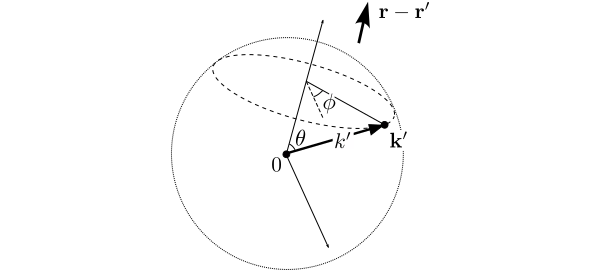
\includegraphics[width=0.4\textwidth]{spherical_coords}
\end{figure}

Then,
\begin{align}
  \langle\mathbf{r}|\hat{G}_0|\mathbf{r}'\rangle &= \frac{2m}{\hbar^2} \frac{1}{(2\pi)^3} \int d^3k' \; \frac{\exp\left[i\mathbf{k}'\cdot (\mathbf{r}-\mathbf{r}')\right]}{k^2-|\mathbf{k}'|^2} \nonumber \\
  &= \frac{2m}{\hbar^2} \frac{1}{(2\pi)^3} \int_0^\infty dk' \int_0^\pi d\theta \int_{0}^{2\pi} d\phi \;{k'}^{2}\sin\theta\; \frac{\displaystyle \exp\left(ik'|\mathbf{r}-\mathbf{r}'|\cos\theta\right)}{k^2-{k'}^2} \nonumber \\
  &= \frac{2m}{\hbar^2} \frac{1}{(2\pi)^2} \int_0^\infty dk' \int_{-1}^1 d\mu \;{k'}^2\; \frac{\displaystyle \exp\left(ik'|\mathbf{r}-\mathbf{r}'|\mu\right)}{k^2-{k'}^2} \qquad(\text{letting}\;\mu = \cos\theta) \nonumber \\
  &= \frac{2m}{\hbar^2} \frac{1}{(2\pi)^2} \int_0^\infty dk' \; \frac{ {k'}^2}{k^2-{k'}^2}\, \frac{\displaystyle \exp\left(ik'|\mathbf{r}-\mathbf{r}'|\right) - \exp\left(-ik'|\mathbf{r}-\mathbf{r}'|\right)}{ik'|\mathbf{r}-\mathbf{r}'|} \nonumber\\
  &= \frac{2m}{\hbar^2} \frac{1}{(2\pi)^2} \frac{i}{|\mathbf{r}-\mathbf{r}'|} \int_{-\infty}^\infty dk' \; \frac{\displaystyle k'\, \exp\left(ik'|\mathbf{r}-\mathbf{r}'|\right)}{(k' - k)(k'+k)}.
  \label{rGrintegrand}
\end{align}
This looks like something we can handle via contour integration.
However, there's a snag: the integration contour runs over the real
$k'$ line, but since $k \in \mathbb{R}^+$, the poles at $\pm k$ lie on
the contour.  The integral, as currently defined, is singular.

To get a proper result, we must ``regularize'' the integral by
tweaking its definition.  One way is to perturb the integrand and
shift its poles infinitesimally in the complex plane, moving them off
the contour.  We have a choice of whether to move each pole
infinitesimally up or down.  It turns out that the appropriate choice
is to shift the pole at $-k$ down, and shift the pole at $+k$ up, as
illustrated by the red dots in the following figure:

\begin{figure}[h!]
  \centering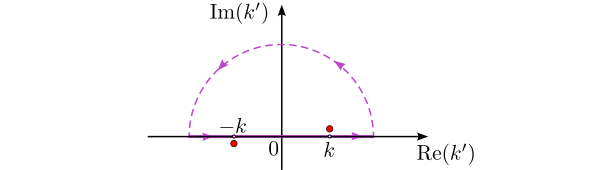
\includegraphics[width=0.37\textwidth]{greencontour}
\end{figure}

\noindent
This choice, which will yield a causal Green's function (Section 1.7),
alters the denominator in the integrand of Eq.~\eqref{rGrintegrand} as
follows:
\begin{equation}
  (k' - k)(k'+k) \;\rightarrow\; (k' - k - i\varepsilon)(k'+k+i\varepsilon) = {k'}^2 - (k+i\varepsilon)^2,
\end{equation}
where $\varepsilon$ is a positive infinitesimal.  This is equivalent
to replacing $E \rightarrow E + i\varepsilon$ in the definition of the
Green's function.  We can now do the integral:
\begin{align*}
  \begin{aligned}\int_{-\infty}^\infty dk' \; \frac{\displaystyle k' \exp\left(ik'|\mathbf{r}-\mathbf{r}'|\right)}{(k' - k)(k'+k)} &\rightarrow \lim_{\varepsilon \rightarrow 0^+} \int_{-\infty}^\infty dk' \; \frac{\displaystyle k' \exp\left(ik'|\mathbf{r}-\mathbf{r}'|\right)}{(k' - k - i\varepsilon)(k'+k+i\varepsilon)}\;\;\; (\text{regularize}) \\ &= \lim_{\varepsilon \rightarrow 0^+} \int_C dk' \; \frac{\displaystyle k' \exp\left(ik'|\mathbf{r}-\mathbf{r}'|\right)}{(k' - k - i\varepsilon)(k'+k+i\varepsilon)} \quad\;\;\; (\text{close contour above}) \\ &= 2\pi i \lim_{\varepsilon \rightarrow 0^+} \mathrm{Res}\left[\frac{\displaystyle k' \exp\left(ik'|\mathbf{r}-\mathbf{r}'|\right)}{(k' - k - i\varepsilon)(k'+k+i\varepsilon)}, \;k'=k+i\varepsilon^+\right] \\ &= \pi i \exp\left(ik|\mathbf{r}-\mathbf{r}'|\right).\end{aligned}
\end{align*}
Plugging this into Eq.~\eqref{rGrintegrand} gives the result
\begin{equation}
  \langle\mathbf{r}|\hat{G}_0|\mathbf{r}'\rangle = -\frac{2m}{\hbar^2}
  \cdot \frac{\exp\left(ik|\mathbf{r}-\mathbf{r}'|\right)}{4\pi|\mathbf{r}-\mathbf{r}'|},
\end{equation}
which is a spherical wave propagating isotropically outward from
$\mathbf{r} = \mathbf{r}'$.  The wave is isotropic because it is
generated by a delta function, which has no preferred direction.  It
is outgoing due to our preceding choice of regularization.

The propagators for other spatial dimensions are listed in Section
1.7.  The 1D and 2D derivations are similar to the above 3D
derivation.  The 2D case is given as an
\hyperref[ex:2dpropagator]{exercise}, with some hints provided.

\section{Scattering relations}
\label{sec:scattering}

Circular waves (Section~\ref{circular_waves}) and spherical waves
(Section~\ref{sec:spherical}) play an important role in the analysis
of scattering problems.

Let $\psi(\mathbf{r})$ be the wavefunction in the external region of a
scattering experiment, where the scattering potential vanishes.  As
described in Chapter 1, $\psi(\mathbf{r})$ obeys the Helmholtz
equation.  We can therefore expand it as a superposition of incoming
and outgoing circular waves (for 2D) or spherical waves (for 3D):
\begin{equation}
  \psi(\mathbf{r}) =
  \left\{
  \begin{aligned}
    &\sum_{m=-\infty}^\infty
    \Big[c_m^+ H_m^+(kr) + c_m^- H_m^-(kr)\Big] \, e^{im\phi}
    & (\textrm{2D})
    \\
    &\sum_{\ell = 0}^\infty \sum_{m = - \ell}^\ell
    \Big[c_{\ell m}^+ h_\ell^+(kr) + c_{\ell m}^- h_\ell^-(kr)\Big] \,
    Y_{\ell m}(\theta, \phi). & (\textrm{3D})
  \end{aligned}\right.
  \label{psirdecomp}
\end{equation}
Since the individual circular or spherical waves satisfy the Helmholtz
equation, which is linear, any such linear superposition automatically
satisfies the Helmholtz equation.  For simplicity, let us denote the
coefficients by $\{c_\mu^\pm\}$, where $\mu \equiv m$ for 2D and $\mu
\equiv (\ell, m)$ for 3D.  Each $\mu$ is called a \textbf{scattering
  channel}.

The circular and spherical waves are appropriately normalized such
that the energy flux carried in scattering channel $\mu$ is directly
proportional to $|c_\mu^\pm|^2$.  This follows from the normalization
choice in the definitions of the Hankel and spherical Hankel
functions, which give rise to the large-$r$ asymptotic forms in
\eqref{Jasymptote} and \eqref{sphJasymptote}.

In a scattering problem, the incoming coefficients $|c_\mu^-|^2$ and
the outgoing coefficients $|c_\mu^+|^2$ are not independent.  Since
the Schr\"odinger wave equation is linear, there must be some linear
relation between them, of the form
\begin{equation}
  c_{\mu}^+ = \sum_{\nu} S_{\mu \nu} \, c_{\nu}^-, \;\;\;\text{for all}\;\;\mu.
  \label{srelation}
\end{equation}
Here, the outgoing wave coefficients are on the left, and the incoming
coefficients on the right.  The complex matrix $S$, called the
\textbf{scattering matrix}, is determined by the scattering potential
$V(\mathbf{r})$ and energy $E$.  It specifies how the scatterer
converts incoming waves into outgoing waves.

Do not confuse these ``incoming'' and ``outgoing'' waves with the
``incident'' and ``scattered'' waves defined in the scattering
problem.  As discussed in Chapter 1, a scattering experiment typically
has an incident wave that is a plane wave, of the form
\begin{equation}
  \psi_i(\mathbf{r}) = \Psi_i \, e^{i\mathbf{k}_i\cdot\mathbf{r}} \;\;\;
  \mathrm{where}\;\; |\mathbf{k}_i| = k.
\end{equation}
However, relative to a given coordinate origin ($r = 0$), a plane wave
is neither purely incoming nor outgoing!  For 2D, we can use
Eq.~\eqref{eikrcosphi} to decompose the plane wave as
\begin{equation}
  \psi_i(\mathbf{r})
  = \frac{\Psi_i}{2} \sum_{m=-\infty}^\infty i^m e^{im \Delta\phi} \,
  \left[H_m^+(kr) + H_m^-(kr)\right],
  \label{psii_2d}
\end{equation}
where $r = |\mathbf{r}|$ and $\Delta \phi =
\cos^{-1}\left[(\mathbf{k}_i\!\cdot\!\mathbf{r})/kr\right]$.
Likewise, for 3D we can use Eq.~\eqref{plane_wave_decomp} to write
\begin{equation}
  \psi_i(\mathbf{r})
  = 2\pi \Psi_i \sum_{\ell=0}^\infty \sum_{m=-\ell}^\ell
  \left[h_{\ell}^+(kr) + h_{\ell}^-(kr) \right] \, e^{i\ell\pi/2} \,
  Y_{\ell m}^*(\hat{\mathbf{k}}_i) \, Y_{\ell m}(\hat{\mathbf{r}}),
  \label{psii_3d}
\end{equation}
where $\hat{\mathbf{k}}_i$ and $\hat{\mathbf{r}}$ denote the angular
components of $\mathbf{k}_i$ and $\mathbf{r}$ respectively.  In both
cases, the incident plane wave is evidently a superposition of
incoming \textit{and} outgoing waves.

Using Eqs.~\eqref{psii_2d} and \eqref{psii_3d}, we will be able to
relate the scattering matrix to the formulation of the scattering
problem discussed in Chapter 1.  Let us see how this is done for 3D;
the 2D case is left as an \hyperref[ex:2dscattering]{exercise}.

Focusing now on 3D, a comparison of Eqs.~\eqref{psirdecomp} and
\eqref{psii_3d} allows us to determine the spherical wave coefficients
for the incident wave:
\begin{equation}
  c^{\pm}_{i, \ell m} = 2 \pi e^{i\ell\pi/2} \,
  Y_{\ell m}^*(\hat{\mathbf{k}}_i)\; \Psi_i.
  \label{cilm}
\end{equation}
The total wavefunction consists of $\psi_i(\mathbf{r})$ plus the
scattered wavefunction $\psi_s(\mathbf{r})$.  By assumption, the
latter is a superposition of only outgoing waves, so denote its
coefficients by $c^+_{s,\ell m}$.  Next, re-express the scattering
matrix equation \eqref{srelation} using these coefficients:
\begin{equation}
  c^+_{i,\ell m} + c^+_{s,\ell m}
  = \sum_{\ell, m, \ell', m'} S_{\ell m, \ell'm'} c^-_{i,\ell'm'}.
\end{equation}
Note that the scattered wave does not contribute to the right side
because it has no incoming components.  Moving $c_{i,\ell m}^+$ to the
right side of the equation, and using Eq.~\eqref{cilm}, gives
\begin{equation}
  c^+_{s,\ell m} = 2 \pi \sum_{\ell' m'} \Big(S_{\ell m, \ell' m'}
  - \delta_{\ell \ell'}\delta_{mm'}\Big) e^{i\ell'\pi/2} \,
  Y_{\ell' m'}^*(\hat{\mathbf{k}}_i)\; \Psi_i.
\end{equation}
Hence, the scattered wavefunction is
\begin{equation}
  \begin{aligned}\psi_s(\mathbf{r}) &= \sum_{\ell m} c^+_{s,\ell m} h_{\ell}^+(kr) \, Y_{\ell m}(\hat{\mathbf{r}}) \\ &= \Psi_i \sum_{\ell m} \sum_{\ell' m'} 2 \pi \Big(S_{\ell m, \ell' m'} - \delta_{\ell \ell'}\delta_{mm'}\Big) e^{i\ell'\pi/2} \, Y_{\ell' m'}^*(\hat{\mathbf{k}}_i)\; h_{\ell}^+(kr) \, Y_{\ell m}(\hat{\mathbf{r}}).\end{aligned}
\end{equation}
For large $r$, we can simplify the spherical Hankel functions using
Eq.~\eqref{sphJasymptote}, obtaining
\begin{equation}
  \psi_s(\mathbf{r}) \overset{r\rightarrow\infty}{\longrightarrow} \, \Psi_i \frac{e^{ikr}}{r} \; \left[ \frac{2 \pi}{ik}\, \sum_{\ell m} \sum_{\ell' m'} \Big(S_{\ell m, \ell' m'} - \delta_{\ell \ell'}\delta_{mm'}\Big) \, e^{-i(\ell-\ell')\pi/2} \, Y_{\ell' m'}^*(\hat{\mathbf{k}}_i)\; Y_{\ell m}(\hat{\mathbf{r}})\right].
\end{equation}
The quantity in square brackets is the scattering amplitude (Section
1.5):
\begin{equation}
  f(\mathbf{k}_i \rightarrow k\hat{\mathbf{r}}) =  \frac{2 \pi}{ik}\, \sum_{\ell m} \sum_{\ell' m'} \Big(S_{\ell m, \ell' m'} - \delta_{\ell \ell'}\delta_{mm'}\Big) \, e^{-i(\ell-\ell')\pi/2} \, Y_{\ell' m'}^*(\hat{\mathbf{k}}_i)\; Y_{\ell m}(\hat{\mathbf{r}}).
  \label{3dfrelation}
\end{equation}

\section{Isotropic scattering potentials}

The scattering relations derived in the previous section can be
greatly simplified if the scattering potential is isotropic,
i.e.~$V(\mathbf{r}) = V(r)$.  In that case, angular momentum is
conserved, so an incoming wave with definite angular momentum must
scatter exclusively into an outgoing wave of the same angular
momentum.  The scattering matrices thus have the form
\begin{align}
  \begin{aligned}
  S_{mm'} &= s_{m}\, \delta_{mm'} && (\text{2D}) \\
  S_{\ell m, \ell'm'} &= s_{\ell m}\, \delta_{\ell\ell'}\, \delta_{mm'}.
  && (\text{3D})
  \end{aligned}
  \label{Ssimple}
\end{align}

In the following, we will focus on the 3D case (the 2D case is handled
similarly).  Plugging Eq.~\eqref{Ssimple} into
Eq.~\eqref{3dfrelation}, we obtain
\begin{equation}
  f(\mathbf{k}_i \rightarrow k\hat{\mathbf{r}}) =  \frac{2 \pi}{ik}\, \sum_{\ell m} \Big(s_{\ell m} - 1\Big) \, Y_{\ell m}^*(\hat{\mathbf{k}}_i)\; Y_{\ell m}(\hat{\mathbf{r}}).
\end{equation}
We now want to find the $s_{\ell m}$'s in terms of the scattering
potential.  The total wavefunction satisfies the Schr\"odinger wave
equation, which can be written in spherical coordinates as
\begin{equation}
  \frac{1}{r^2}\frac{\partial}{\partial r}\left(r^2\frac{\partial \psi}{\partial r}\right) + \frac{1}{r^2\sin\theta}\frac{\partial}{\partial\theta}\left(\sin\theta\frac{\partial\psi}{\partial\theta}\right)+\frac{1}{r^2\sin^2\theta}\frac{\partial^2\psi}{\partial\phi^2} + K^2(r) \psi(r,\theta,\phi) = 0,
\end{equation}
where
\begin{equation}
  K^2(r) = \sqrt{\frac{2m\big[E-V(r)\big]}{\hbar^2}}.
\end{equation}
This is similar to the Helmholtz equation, but with the constant $k^2$
replaced by a function $K^2(r)$.  In scattering channel $(\ell,m)$,
the solution has the form
\begin{equation}
  \psi(r,\theta,\phi) = A(r) \, Y_{\ell m}(\theta, \phi).
\end{equation}
Upon substitution into the Schr\"odinger wave equation, we find that
$A(r)$ must satisfy
\begin{equation}
  \frac{d}{dr}\left(r^2\frac{dA}{dr}\right) + \Big[K^2(r)\, r^2 - \ell(\ell+1)\Big] A(r) = 0, \;\;\;\ell \in \mathbb{Z}_0^+.
\end{equation}
As before, the equation for $A(r)$ does not involve $m$; hence, the
scattering matrix components do not depend on $m$, and can be written
as simply
\begin{equation}
  s_{\ell m} \,=\, s_\ell.
\end{equation}
For any given $V(r)$, we can solve the second-order ordinary
differential equation numerically by supplying two boundary conditions
at $r=0$, integrating up to a large value of $r$, and matching to the
exterior solution
\begin{equation}
  A(r) \; \overset{r\rightarrow\infty}{\longrightarrow} \; c^-_\ell h^-_\ell(kr) + c^+_\ell h^+_\ell(kr) = c^-_\ell \Big(h^-_\ell(kr) + s_\ell h^+_\ell(kr)\Big).
\end{equation}
The value of $s_\ell$ can then be extracted.

To simplify the problem even further, let the scattering potential
take the form of a spherical potential well of radius $R$ and depth
$U$:
\begin{equation}
  V(r) = \begin{cases}-U &\mathrm{for}\;\; r < R, \\ \;\;\; 0 & \mathrm{otherwise}.\end{cases}
\end{equation}
We will take $U > 0$, so that the potential is attractive.  (The
interested reader can work through the repulsive case, $U < 0$.  The
process is almost the same as what is presented below, except that for
some values of $E$, the wave inside the scatterer becomes evanescent.)
Now, the Schr\"odinger wave equation in the interior region reduces to
the Helmholtz equation, but with $k$ replaced with
\begin{equation}
  q = \sqrt{2m(E+U)/\hbar^2}.
\end{equation}
Note that $q \in \mathbb{R}^+$ for $E > 0$, since we have assumed
that $U > 0$.  The elementary solutions for $A(r)$ in the interior
region are $j_\ell(qr)$ and $y_\ell(qr)$.  However, we must exclude
the latter, since they diverge at $r = 0$.  (When we got to a similar
point in Section~\ref{sec:spherical}, we did not exclude the spherical
Bessel functions of the second kind, because at the time we were
concerned with solutions in the exterior region.)  We thus arrive at a
solution of the form
\begin{equation}
  A(r) = \begin{cases} \alpha_\ell\, j_\ell(qr), & r \le R \\ c^-_\ell \Big(h^-_\ell(kr) + s_\ell h^+_\ell(kr)\Big) & r \ge R.\end{cases}
\end{equation}
So far, the values of $\alpha_\ell$, $c^-_\ell$, and $s_\ell$ remain
unknown.  To proceed, we match the wavefunction and its
derivative at the boundary $r = R$:
\begin{align}
  \begin{aligned} \alpha_\ell\, j_\ell(qR) &= c^-_\ell \Big(h^-_\ell(kR) + s_\ell h^+_\ell(kR)\Big) \\ \alpha_\ell\, q j_\ell'(qR) &= c^-_\ell k \Big({h^-_\ell}'(kR) + s_\ell {h^+_\ell}'(kR)\Big).\end{aligned}
\end{align}
Here, $j_\ell'$ denotes the derivative of the spherical Bessel
function, and likewise for ${h_\ell^\pm}'$.  Taking the ratio of these
two equations eliminates $\alpha_\ell$ and $c_\ell^-$:
\begin{equation}
  \frac{q j_\ell'(qR)}{j_\ell(qR)} = k \frac{{h^-_\ell}'(kR) + s_\ell {h^+_\ell}'(kR)}{h^-_\ell(kR) + s_\ell h^+_\ell(kR)}.
\end{equation}
With a bit of rearrangement, this becomes
\begin{equation}
  s_\ell = - \frac{k{h_\ell^-}'(kR) j_\ell(qR) - qh_\ell^-(kR)j_\ell'(qR)}{k{h_\ell^+}'(kR) j_\ell(qR) - qh_\ell^+(kR)j_\ell'(qR)}.
\end{equation}
The numerator and denominator are complex conjugates of one another,
since $j_\ell$ is real and $(h_\ell^+)^* = h_\ell^-$.  Hence,
\begin{equation}
  s_\ell = e^{2i\delta_\ell}, \;\;\;\mathrm{where}\;\; \delta_\ell = \frac{\pi}{2} - \mathrm{arg}\!\left[k{h_\ell^+}'(kR) j_\ell(qR) - qh_\ell^+(kR)j_\ell'(qR)\right].
\end{equation}
In other words, the scattering matrix component is a pure phase
factor.  This is actually a consequence of energy conservation.  Since
the scattering matrix does not couple different angular momentum
channels (due to the spherical symmetry), the incoming flux and
outgoing flux in each channel must be equal.  Hence, the only thing
the scattering potential can do is to shift the phase of the outgoing
spherical wave component in each channel.

Once we find $\delta_\ell$, we can compute the scattering amplitude
\begin{equation}
  f(\mathbf{k}_i\rightarrow k\hat{\mathbf{r}}) = \frac{2 \pi}{ik}\, \sum_{\ell =0}^\infty \big(e^{2i\delta_\ell} - 1\big) \, \sum_{m=-\ell}^\ell \,Y_{\ell m}^*(\hat{\mathbf{k}}_i)\; Y_{\ell m}(\hat{\mathbf{r}}).
\end{equation}
This can be simplified with the aid of the following addition theorem
for spherical harmonics:
\begin{equation}
  P_\ell(\hat{\mathbf{r}}_1\cdot\hat{\mathbf{r}}_2) = \frac{4\pi}{2\ell+1} \sum_{m=-\ell}^{\ell} Y_{\ell m}^*(\hat{\mathbf{r}}_1) Y_{\ell m}(\hat{\mathbf{r}}_2).
\end{equation}
where $P_\ell(\cdots)$ denotes a
\href{https://en.wikipedia.org/wiki/Legendre_polynomials}{Legendre
  polynomial}.  We finally obtain
\begin{equation}
  \boxed{\quad\begin{aligned}f(\mathbf{k}_i \rightarrow k\hat{\mathbf{r}}) &= \frac{1}{2ik}\, \sum_{\ell =0}^\infty \big(e^{2i\delta_\ell} - 1\big) \big(2\ell+1\big)\, P_{\ell}(\hat{\mathbf{k}}_i\cdot \hat{\mathbf{r}}) \\ \delta_\ell &= \frac{\pi}{2} - \mathrm{arg}\!\left[k{h_\ell^+}'(kR) \, j_\ell(qR) - qh_\ell^+(kR)\, j_\ell'(qR)\right] \\ k &= |\mathbf{k}_i| = \sqrt{2mE/\hbar^2}, \;\; q = \sqrt{2m(E+U)/\hbar^2}.\end{aligned}\quad}
\end{equation}
This result for the scattering amplitude depends upon two variables:
(i) $E$, the particle energy (which is conserved), and (ii) $\Delta
\theta = \cos^{-1}(\hat{\mathbf{k}}_i\cdot \hat{\mathbf{r}})$, the
\textbf{deflection angle} (i.e., the angle between the direction of
incidence and the direction into which the particle is scattered).

\section*{Exercises}

\begin{enumerate}
\item \label{ex:2dpropagator}
  In Section~\ref{sec:propagator}, we derived the 3D propagator.
  Using a similar procedure, prove that the 2D propagator is
  \begin{equation}
    \langle\mathbf{r}|\hat{G}_0|\mathbf{r}'\rangle = \frac{2m}{\hbar^2}\;
    \cdot\; \frac{1}{4i} H^+_0(k|\mathbf{r}-\mathbf{r'}|).
  \end{equation}
  In evaluating the polar integral, you may find it useful to invoke
  Eq.~\eqref{eikrcosphi}.  To solve the resulting contour integral,
  you may refer to the asymptotic forms of the Bessel and Hankel
  functions given in \eqref{Jasymptote}, and the identity
  \begin{equation}
    H_m^+(z) = - (-1)^m \, H_m^-(-z).
  \end{equation}

\item \label{ex:2dscattering} In Section~\ref{sec:scattering}, we
  derived an expression for the 3D scattering amplitudes in terms of
  the scattering matrix $S$, Eq.~\eqref{3dfrelation}.  Starting from
  Eq.~\eqref{psii_2d}, derive the corresponding relation for the 2D
  scattering amplitudes.

\end{enumerate}

\end{document}
